\subsection{Control to voltage}
\label{subsec:control_to_voltage}

As already clarified in Section \ref{subsubsec:control_input_correction}, what we actually control is the duty cycle of the PWM signal that is applied to the coils.
However, as we saw in Equation \ref{eq:reduced_equations_of_motion}, the model consider the effective voltage applied to the coils as input.

In order to use the control signal as input to the model, we need to identify the parameters of the relation between the control signal and the effective voltage applied to the coils which has already been discussed in Equation \ref{eq:voltage_duty_cycle_relation}.

The experimental procedure to identify this relation can be summarized in the following steps:

\begin{enumerate}
    \item Connect the control unit to the coils and to the power supply.
    \item Connect the multimeter to the coils and set it to measure the voltage.
    \item Set the control unit to a specific duty cycle.
    \item Measure the voltage applied to the coils.
    \item Repeat steps 3 and 4 for many duty cycles.
\end{enumerate}

The output of this test is a series of points that can be fitted to \ref{eq:voltage_duty_cycle_relation} in order to identify the parameters of the relation.
In Figure \ref{fig:control_to_voltage} we can observe both the measured points, the linear fitting and the effective voltage applied considering also the initial black zone.

\begin{figure}[H]
    \centering
    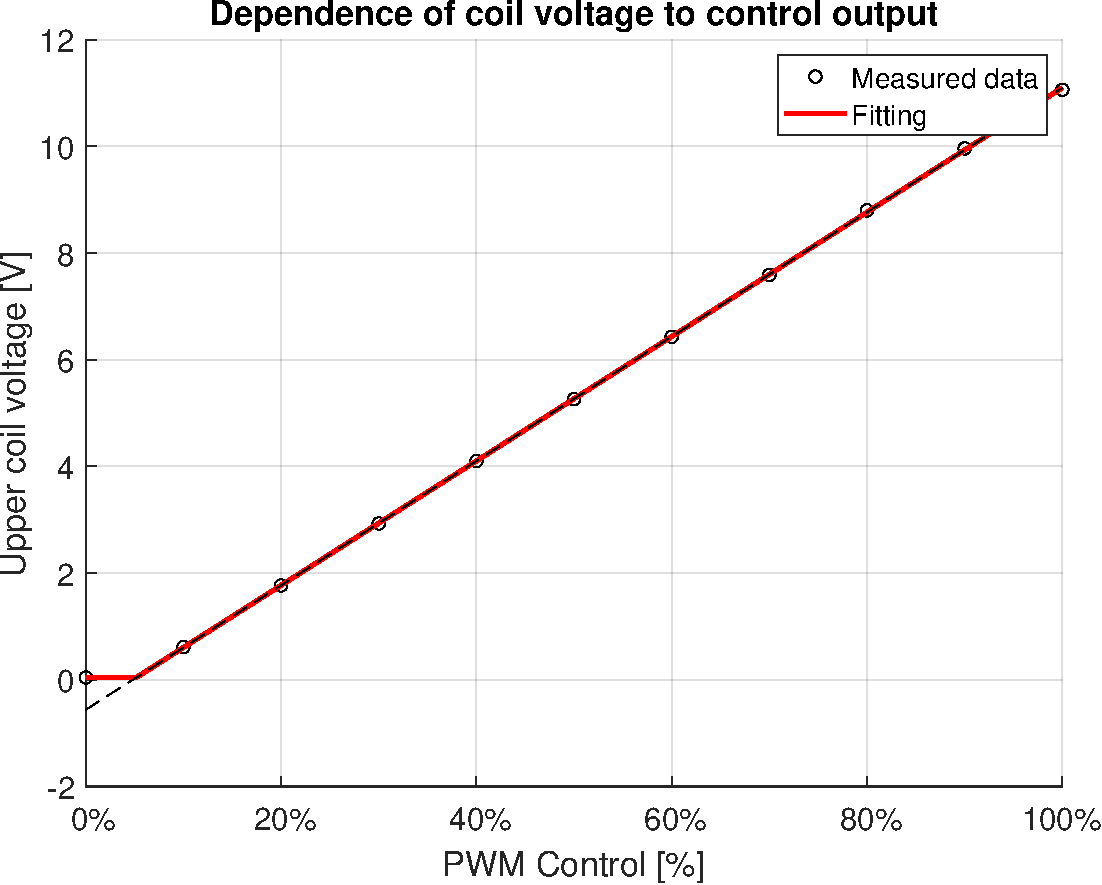
\includegraphics[width=0.6\textwidth]{img/MATLAB/identification/control_to_voltage.pdf}
    \caption{Control to voltage identification}
    \label{fig:control_to_voltage}
\end{figure}

As we can see, the linear model for the relation $V = f(U) = f(\text{PWM})$ is a good approximation outside the initial black zone control.

The values of the parameters for the Equation \ref{eq:voltage_duty_cycle_relation} are shown in Table \ref{tab:control_to_voltage_parameters}.
One might refer to Section \ref{subsubsec:control_input_correction} for an explanation of the parameters.

\begin{table}[H]

    \centering
    \begin{tabular}{|c|c|c|}
        \hline
        \textbf{Parameter} & \textbf{Value}            & \textbf{Units} \\
        \hline
        $V_{min}$          & $4.300000 \cdot 10^{-2}$  & $V$            \\
        $U_{min}$          & $5.179276$                & $\%$           \\
        $k$                & $1.165800 \cdot 10^{1}$   & $V/\%$         \\
        $c$                & $-5.608000 \cdot 10^{-1}$ & $V$            \\
        \hline
    \end{tabular}

    \caption{Control to voltage identification parameters}
    \label{tab:control_to_voltage_parameters}

\end{table}